% 2020 新高考Ⅰ卷（山东）20：四棱锥 P-ABCD（底面 ABCD 为正方形，PD⊥底面 ABCD）
% 绘制依据：固定源 PDF 原页。底面按斜二测画：A 左前、B 右前、C 右后、D 中后（被遮挡顶点）；
% PD 垂直底面，故 P 画在 D 的正上方（位于版面中偏左）。
% 实线：PA、PB、PC、AB、BC；虚线：PD、AD、DC。只标 P、A、B、C、D 五点。
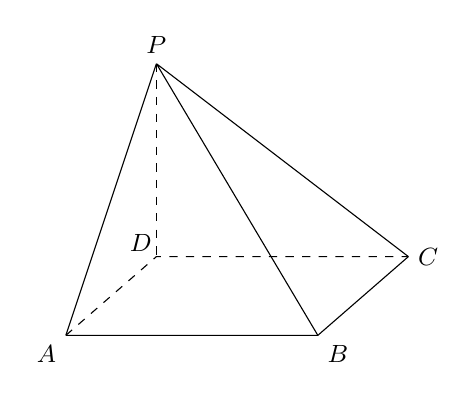
\begin{tikzpicture}[scale=1.0, font=\small]
  \coordinate (A) at (0,0);
  \coordinate (B) at (3.2,0);
  \coordinate (C) at (4.35,1.0);
  \coordinate (D) at (1.15,1.0);
  \coordinate (P) at (1.15,3.45);
  \draw (P) -- (A)  (P) -- (B)  (P) -- (C);
  \draw (A) -- (B) -- (C);
  \draw[dashed] (P) -- (D);
  \draw[dashed] (A) -- (D) -- (C);
  \node[above] at (P) {$P$};
  \node[below left] at (A) {$A$};
  \node[below right] at (B) {$B$};
  \node[right] at (C) {$C$};
  \node[above left, inner sep=1.5pt] at (D) {$D$};
\end{tikzpicture}
